\documentclass[a4paper, 11pt]{article}
\usepackage[margin=0.75in]{geometry}
\usepackage[english]{babel}
\usepackage[utf8]{inputenc}
\usepackage{amsmath}
\usepackage{graphicx}
\usepackage[colorinlistoftodos]{todonotes}
\usepackage{listings}
\usepackage{epstopdf}
\usepackage{import}
\usepackage[none]{hyphenat}
\usepackage{algorithmicx}
\usepackage{algorithm}% http://ctan.org/pkg/algorithms
\usepackage{algpseudocode}% http://ctan.org/pkg/algorithmicx

\usepackage{array}
\newcolumntype{L}[1]{>{\raggedright\let\newline\\\arraybackslash\hspace{0pt}}m{#1}}
\newcolumntype{C}[1]{>{\centering\let\newline\\\arraybackslash\hspace{0pt}}m{#1}}
\newcolumntype{R}[1]{>{\raggedleft\let\newline\\\arraybackslash\hspace{0pt}}m{#1}}

\lstset{basicstyle=\ttfamily,breaklines=true}

\title{User Manual for GDB based debugger for AJIT Multi-core, Multi-threaded Processors

\author{Titto Thomas, Madhav Desai\\Department of Electrical Engg.\\ IIT Bombay, Mumbai}

\date{\today}

\begin{document}
\maketitle

\section{Introduction}

The Ajit processor implements the SPARC V8 instruction set, and 
can be configured with up to four cores, with each core having
either one or two execution threads.  To debug such a processor,
we implement a debug server which can be used to communicate with
the processor threads (either in a C model, or an FPGA prototype).
We use a GDB remote debug client for each of the threads being
debugged.

In this document, we describe the 
process of using GDB remote clients for real-time debug
of the multiple threads in an AJIT processor system.
\begin{itemize}
	\item ISA-C model
	\item Micro-architecture model in C
	\item Micro-architecture VHDL model running in simulator
	\item Micro-architecture model on FPGA prototype
\end{itemize}

\section{Building AJIT processor models}
Throughout the document we will be using repository home to indicate the Ajit project git repository. First go to that directory and run the following commands.

\begin{lstlisting}[language=bash]
$ source exports.sh
$ ./build.sh
\end{lstlisting}
This will build the both processor and ISA-C model executables. For using GDB to debug the programs running on it, you need to use the appropriate one from the following.

\vspace*{5mm}

\begin{tabular}{L{4cm} C{5mm} L{10cm}}
	\hline
	ISA-C model & : & \texttt{AJIT\_cpu\_cache\_mmu\_testbench\_gdbserver}\\ \hline
	Micro-architecture model in C & : & \texttt{ajit\_cpu\_uarch\_test\_gdbserver}\\ \hline
	Micro-architecture VHDL model running in simulator & : & \texttt{ajit\_cpu\_uarch\_test\_gdbserver\_sockpipes}\\ \hline
	Micro-architecture model on FPGA prototype & : & \texttt{ajit\_cpu\_uarch\_test\_gdbserver\_riffa}\\ \hline
\end{tabular}

\section{Creating executables for AJIT}
We are using the cross compiler and gdb that comes along with the buildroot package. The installation instructions are given in \texttt{repository\_home/tools/buildroot/README}. After installing them, go to the directory where your C file is located and run the following command
\begin{lstlisting}[language=bash]
$ cToSparc.py <input file>.c
\end{lstlisting}
An \texttt{output} directory will be created in the same folder with memory map files and executable.

\section{Starting a session of GDB for AJIT}
Go to the directory where your C file was compiled and enter the following command.
\begin{lstlisting}[language=bash]
$ sparc-linux-gdb <input file>.elf
\end{lstlisting}
Now the gdb will start and you can see the messages shown in Fig. 1

\begin{figure}[H]
		\centering
		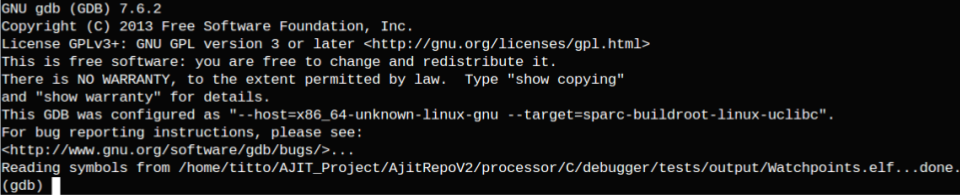
\includegraphics[width=0.8\columnwidth]{Figs/first.png}
		\caption{GDB debug session}
\end{figure}

\textit{Note: The reading symbols from elf file should succeed without any errors}
\\\\
Now, open another tab in the terminal and navigate to \texttt{repository\_home}, run 
\begin{lstlisting}[language=bash]
$ source exports.sh
\end{lstlisting}

and move over to the directory where your C file was compiled. Run the appropriate AJIT processor executable depending on the model to be used.

\subsection*{ISA-C model}
\begin{lstlisting}[language=bash]
$ AJIT_cpu_cache_mmu_testbench_gdbserver <input file>_memmap.txt
<port number>
\end{lstlisting}

\subsection*{Micro-architecture model in C}
\begin{lstlisting}[language=bash]
$ ajit_cpu_uarch_test_gdbserver -m <input file>_memmap.txt
-p <port number>
\end{lstlisting}

\subsection*{Micro-architecture VHDL model running in simulator}
\begin{lstlisting}[language=bash]
$ ajit_cpu_uarch_test_gdbserver_sockpipes -m <input file>_memmap.txt
-p <port number>
\end{lstlisting}
In this case the simulator has to be started as well. Open another tab in the terminal, navigate to\\ \texttt{repository\_home/processor/Aa\_v2/modelsim/vsim\_functional\_check} and run the following script.
\begin{lstlisting}[language=bash]
$ run_modelsim vsim.do
\end{lstlisting}

\subsection*{Micro-architecture model on FPGA prototype}
\begin{lstlisting}[language=bash]
$ ajit_cpu_uarch_test_gdbserver_riffa -m <input file>_memmap.txt
-p <port number>
\end{lstlisting}

\vspace*{1cm}
You can give any of the allowed free ports for \texttt{port number}, preferably 8888.

Now go back to the other tab where gdb is located, and enter the following command with
the same \texttt{port number}.
\begin{lstlisting}[language=bash]
(gdb) target remote :<port number>
\end{lstlisting}

The gdb side will also show the following messages confirming the connection establishment. Since the connection has now been established, you can control and monitor the program execution on AJIT processor in real time.
\begin{figure}[H]
	\centering
	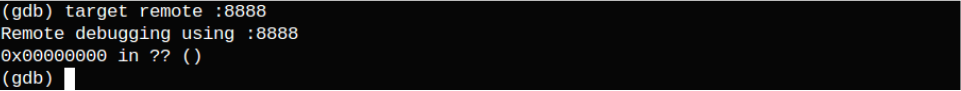
\includegraphics[width=0.8\columnwidth]{Figs/second.png}
\end{figure}

\section*{Basic GDB commands for use}
\subsection*{Continue / Next}
When the execution is stopped due to some reason, you can let the processor continue with these commands.
\begin{lstlisting}[language=bash]
(gdb) continue
(gdb) c
\end{lstlisting}
Next command also lets the processor continue, but stops it after executing one more line of code.
\begin{lstlisting}[language=bash]
(gdb) next
(gdb) n
\end{lstlisting}

\subsection*{Breakpoints}
Breakpoints are useful for stopping the execution on reaching specific points in the source code, and probe the processor for information. They can be set using the following commands.
\begin{lstlisting}[language=bash]
(gdb) break <function_name>
(gdb) break <line_number>
(gdb) break <filename : function_name>
(gdb) break <filename : line_number>
(gdb) break *<address>
\end{lstlisting}
Example:
\\
\begin{figure}[H]
	\centering
	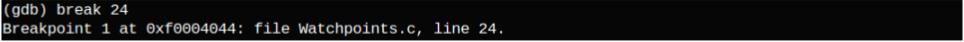
\includegraphics[width=0.8\columnwidth]{Figs/fourth.png}
\end{figure}

AJIT processor will stop execution when a breakpoint is hit, and you will be notified in gdb.
\begin{figure}[H]
	\centering
	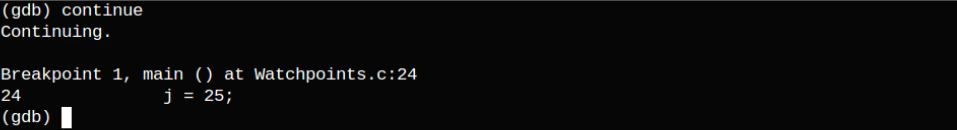
\includegraphics[width=0.8\columnwidth]{Figs/fifth.png}
\end{figure}
Breakpoints can be listed by the following command.
\begin{lstlisting}[language=bash]
(gdb) info breakpoints
\end{lstlisting}

This command can be used to delete specific breakpoints.
\begin{lstlisting}[language=bash]
(gdb) delete break <breakpoint_number>
\end{lstlisting}

\subsection*{Watchpoints}
Breakpoints are useful for stopping the execution on modification of specific variables in the source code, and probe the processor for information. They can be set using the following commands.
This command can be used to delete specific breakpoints.
\begin{lstlisting}[language=bash]
(gdb) watch [-l|-location] <variable>
(gdb) break [-l|-location] <expression>
\end{lstlisting}
Ordinarily a watchpoint respects the scope of variables in expression. The \texttt{-location} argument tells gdb to instead watch the memory referred to by expression.

Example:
\begin{figure}[H]
	\centering
	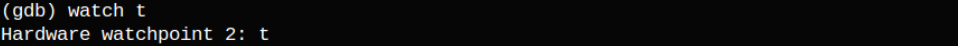
\includegraphics[width=0.8\columnwidth]{Figs/sixth.png}
\end{figure}
AJIT processor will stop execution when a watchpoint is hit, and you will be notified with their values in gdb.
\begin{figure}[H]
	\centering
	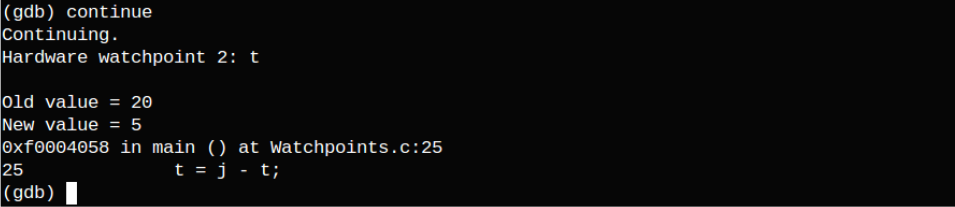
\includegraphics[width=0.8\columnwidth]{Figs/seventh.png}
\end{figure}
Watchpoints can be listed by the following command.
\begin{lstlisting}[language=bash]
(gdb) info watchpoints
\end{lstlisting}

This command can be used to delete specific watchpoints.
\begin{lstlisting}[language=bash]
(gdb) delete watch <watchpoint_number>
\end{lstlisting}

\subsection*{Traps}
While the AJIT processor is executing a program, it will stop and inform the gdb in case of any traps. After it traps, you can use the \texttt{tbr} register to get information about the trap occurred.

Example:
\begin{figure}[H]
	\centering
	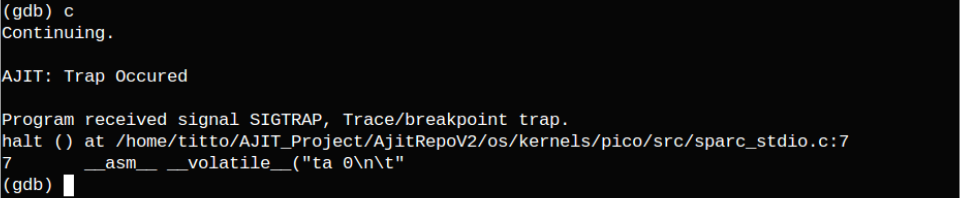
\includegraphics[width=0.8\columnwidth]{Figs/eigth.png}
\end{figure}
\subsection*{Setting variables / memory / registers}
You can modify the values of variables, memory contents and register values with the set command.
\begin{lstlisting}[language=bash]
(gdb) set var <variable> = <value>
(gdb) set $ <register> = <value>
(gdb) set *(int)<memory_address> = <value>
\end{lstlisting}
Example:
\begin{figure}[H]
	\centering
	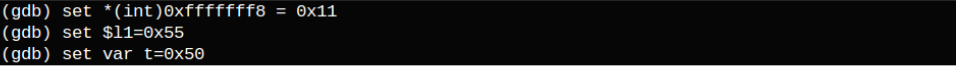
\includegraphics[width=0.8\columnwidth]{Figs/nine.png}
\end{figure}
\subsection*{Printing variables / memory / registers}
You can display the values of variables, memory contents and register values with the \texttt{print} or \texttt{p} command.
\begin{lstlisting}[language=bash]
(gdb) print var <variable>
(gdb) print $ <register>
(gdb) print *(int)<memory_address>
\end{lstlisting}
Example:
\begin{figure}[H]
	\centering
	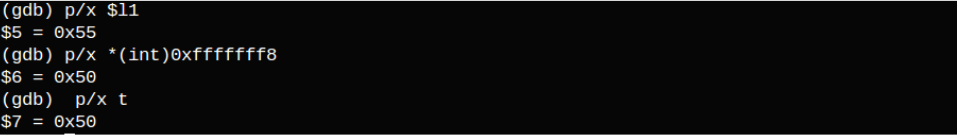
\includegraphics[width=0.8\columnwidth]{Figs/eleven.png}
\end{figure}
\subsection*{Detach}
You can stop debugging the program and let the processor continue till it finishes execution, using this command.
\begin{lstlisting}[language=bash]
(gdb) detach
\end{lstlisting}

Example:
\begin{figure}[H]
	\centering
	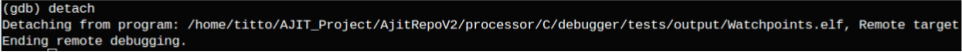
\includegraphics[width=0.8\columnwidth]{Figs/twelve.png}
\end{figure}
\subsection*{Other useful commands}
You can get help on any commands using
\begin{lstlisting}[language=bash]
(gdb) h[elp]
(gdb) h[elp] <command>
\end{lstlisting}
Finish current function, loop, etc. with
\begin{lstlisting}[language=bash]
(gdb) fin[ish]
\end{lstlisting}
Show lines of code surrounding the current point
\begin{lstlisting}[language=bash]
(gdb) l[ist]
\end{lstlisting}
Delete all breakpoints
\begin{lstlisting}[language=bash]
(gdb) d[elete]
\end{lstlisting}
Add a list of gdb commands to execute each time a breakpoint is hit
\begin{lstlisting}[language=bash]
(gdb) comm[ands] <breakpoint_number>
\end{lstlisting}

\end{document}
